\documentclass{article}
\usepackage[utf8]{inputenc}
\usepackage{wasysym}
\usepackage{qrcode}
\usepackage[colorlinks]{hyperref}
\usepackage{listings}
\usepackage{lmodern}
\usepackage{graphicx}
\usepackage{xcolor}
\usepackage[left=2cm, top=3cm, right=2cm]{geometry}
\usepackage{svg}

\definecolor{codebg}{rgb}{0.95, 0.95, 0.95}
\lstset{
  backgroundcolor=\color{codebg},
  basicstyle=\ttfamily\small,
  frame=single,
  breaklines=true,
  keywordstyle=\bfseries\color{blue},
  showstringspaces=false
}

%setup new colors
\hypersetup{
%linkcolor=blue
%,citecolor=
%,filecolor=
urlcolor=blue
%,menucolor=
%,runcolor=
%,linkbordercolor=
%,citebordercolor=
%,filebordercolor=
%,urlbordercolor=
%,menubordercolor=
%,runbordercolor=
}

\title{Database Administration \\ Lab 01: Metadata Tools}
\author{Andrés Calderón, Ph.D.}
\date{\today}

\begin{document}

\maketitle

\section{Introduction}
The main objective of this lab is to explore a database tool for automatically generating a Data Dictionary. \href{https://schemaspy.org/}{SchemaSpy} is a multiplatform DBA tool designed for various DBMS. It is a CLI program that connects to a database and extracts useful information about tables, attributes, and relationships. We will cover a basic guide and then explore other similar tools as independent work.

\section{SchemaSpy Tutorial}

\begin{enumerate}
    \item First, we will download SchemaSpy v6.2.4 from \href{https://github.com/schemaspy/schemaspy/releases/tag/v6.2.4}{here}. SchemaSpy is a Java application, so ensure that you have a stable JRE installed on your system. If Java is not present or if you want to update or change the current installation, follow the steps in \href{https://www.linuxcloudvps.com/blog/install-java-lts-on-ubuntu-24-04/}{this} tutorial.
 
    \item To perform this lab, we need a dummy database to analyze, so we will use the Motor Race Database (MRD), available \href{https://github.com/aocalderon/ergast-mrd}{here}, which contains data about Formula 1 races. An Entity-Relationship Diagram can be seen in Figure \ref{fig:erd}, and a PostgreSQL dump file of the database can be downloaded \href{https://drive.google.com/file/d/1ARHlgpcgQ0nddTUFsQqdevDfFYbGPd6d/view?usp=sharing}{here}.

    \begin{figure}[t]
        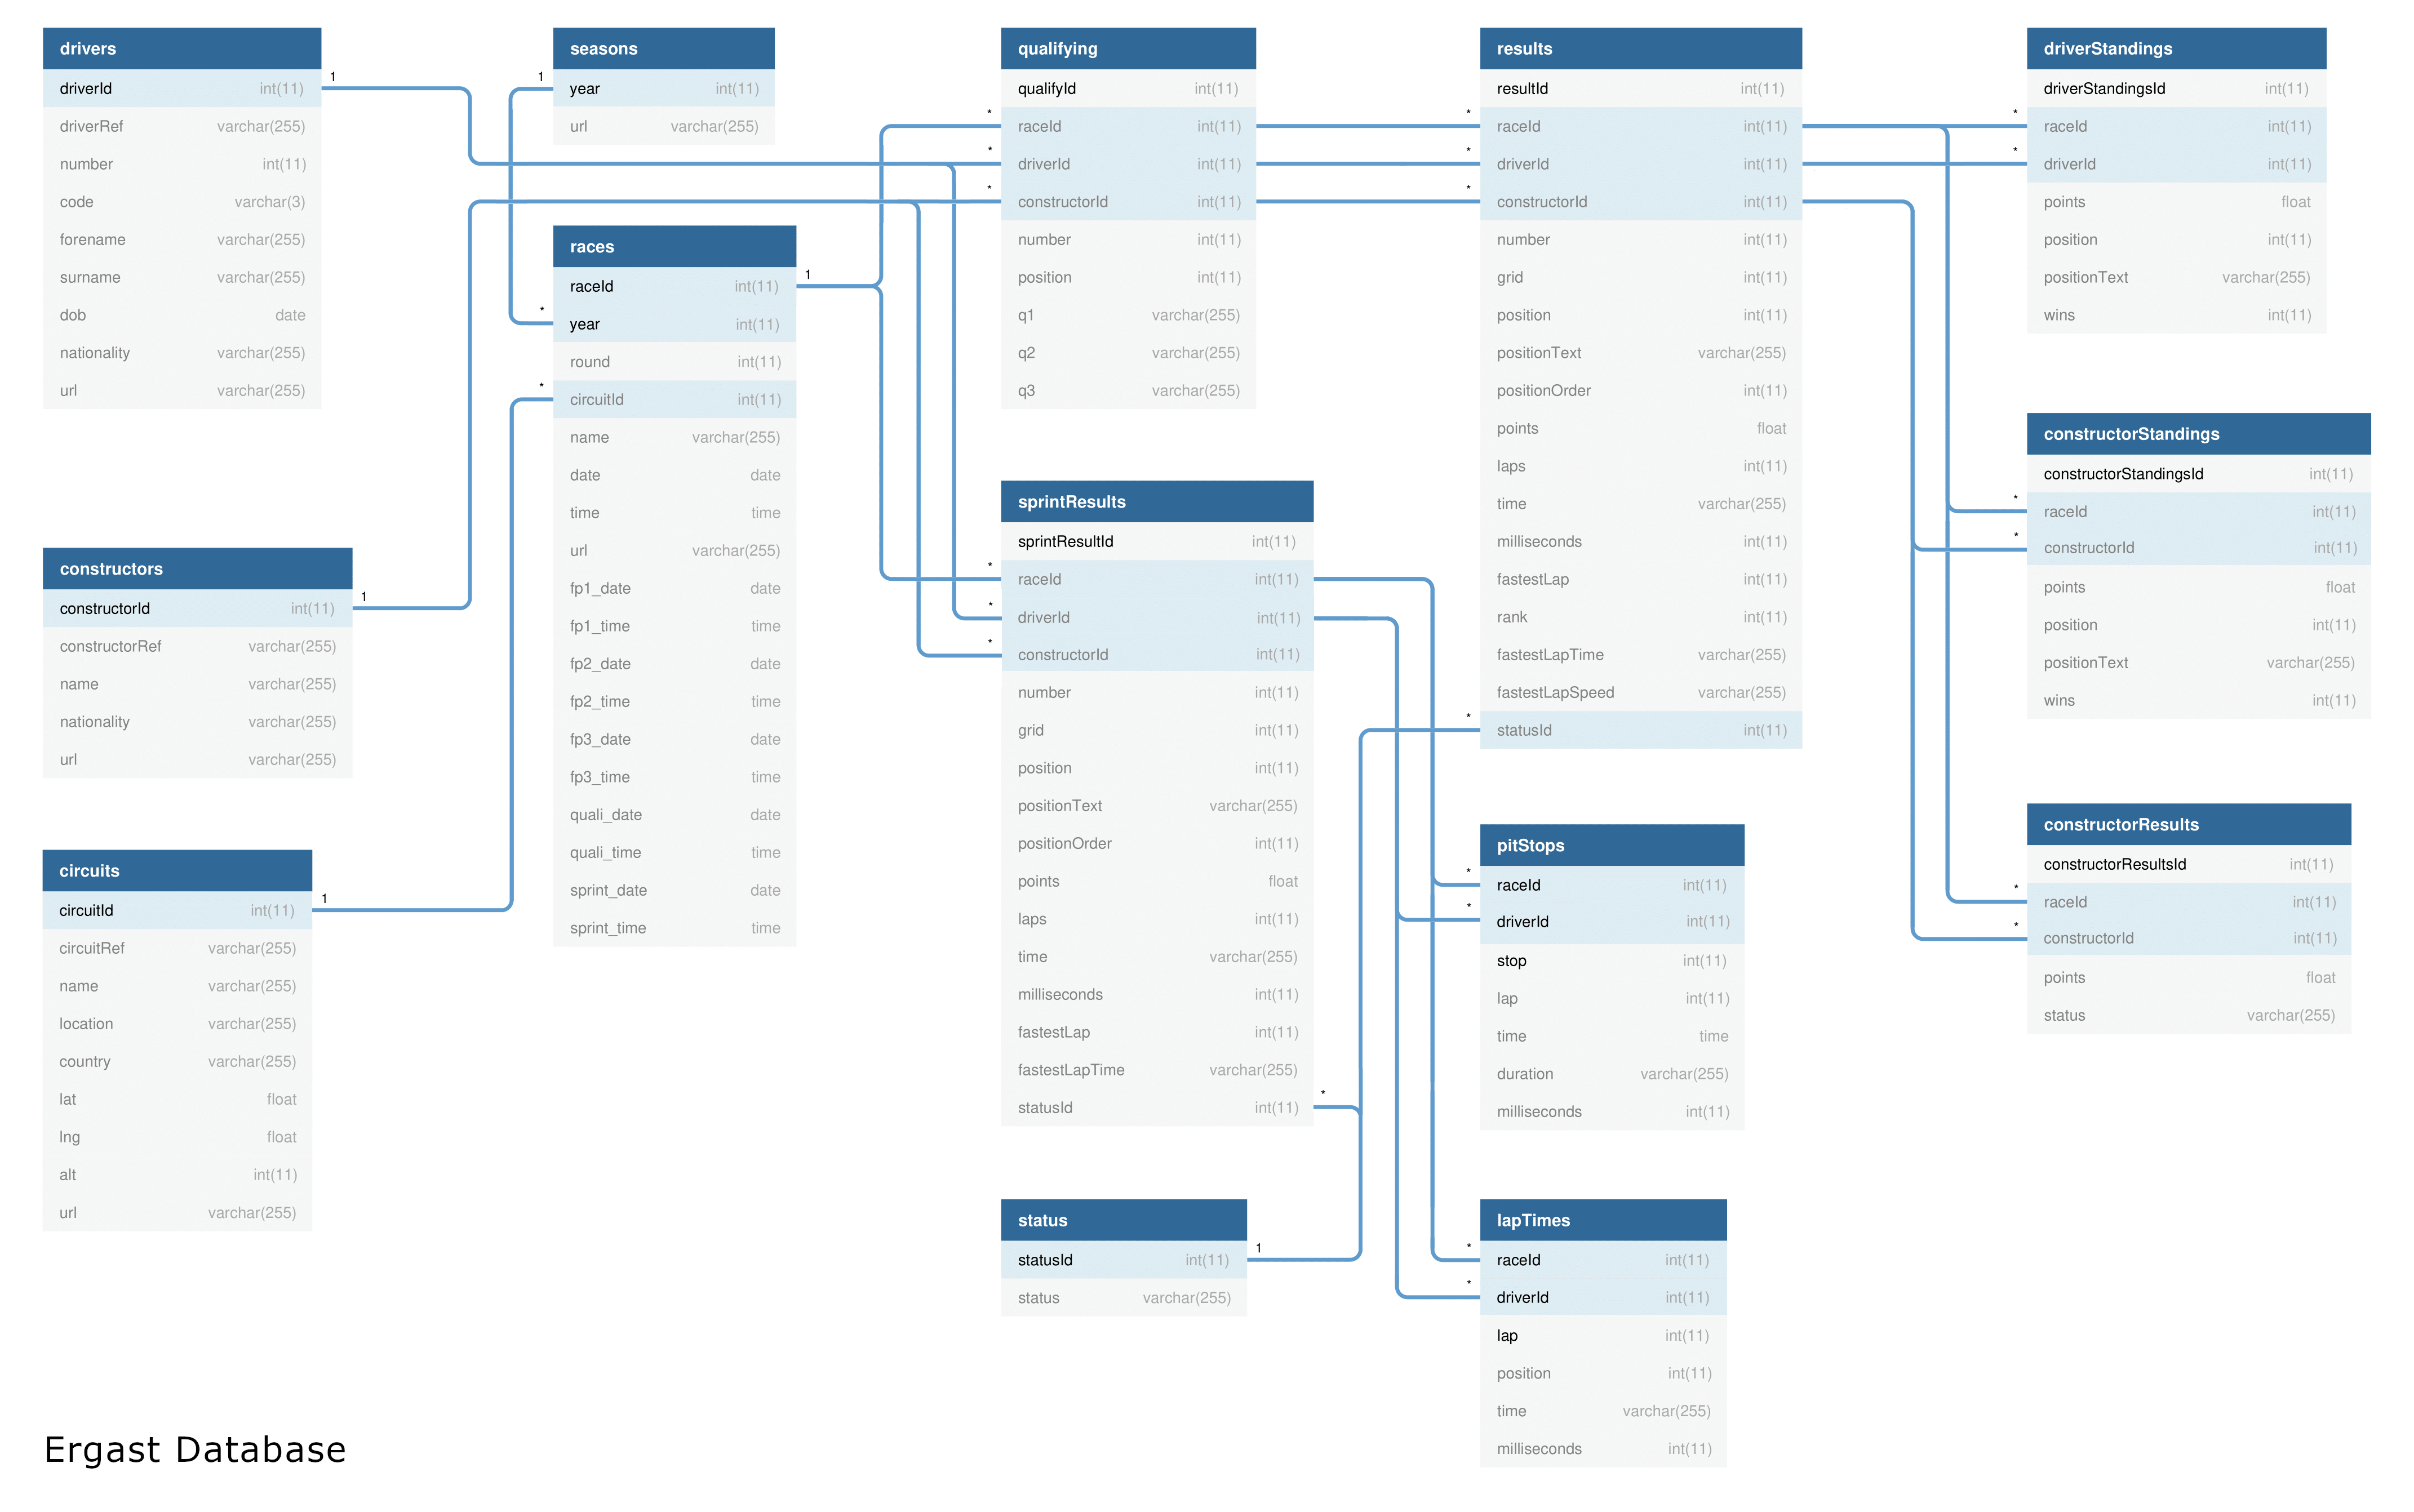
\includegraphics[width=\textwidth]{figures/mrd.png}
        \caption{The E-R Diagram of the MRD.}
        \label{fig:erd}
    \end{figure}

    To upload the sample database, create a PostgreSQL database named \texttt{mrd} in a console while logged in as your Linux user:
 
    \begin{lstlisting}[language=bash]
    $ createdb mrd
    \end{lstlisting}

    Connect to the sample database using the following command:

    \begin{lstlisting}[language=bash]
    $ psql mrd
    \end{lstlisting}

    From the PostgreSQL prompt (once you are in the PostgreSQL environment), upload the dump file using the following command: \texttt{\textbackslash i \textit{path\_to\_dump\_file}}

    \begin{lstlisting}[language=bash]
    mrd=# \i dump_mrd.sql
    \end{lstlisting}

    You may need to adjust the full path of the file as necessary.

    \item To connect to a particular DBMS, we need a \underline{J}ava \underline{D}ata\underline{B}ase \underline{C}onnector (JDBC) for that specific DBMS. Since we are working with PostgreSQL, we need to download the official PostgreSQL JDBC driver from \url{https://jdbc.postgresql.org/}.

    At the time of writing, the current version is 42.7.7, so you should download a file named \texttt{postgresql-42.7.7.jar}. Please place the driver in the same location as the SchemaSpy application.

    \item Next, let's create a folder called \texttt{dd} in the same directory as \texttt{schemaspy} and the JDBC driver to store the results.

    \begin{lstlisting}[language=bash]
    $ mkdir dd
    \end{lstlisting}

    \item Now, we can run the SchemaSpy tool to generate a Data Dictionary from the available data. To do so, type the following command in a terminal console from the folder where the \texttt{schemaspy} executable and the JDBC driver reside:

    \begin{lstlisting}[language=bash]
    $ java -jar schemaspy-6.2.4.jar -t pgsql11 -dp postgresql-42.7.7.jar -db mrd \
            -host localhost -port 5432 -s f1db -u your_username -vizjs -o dd/
    \end{lstlisting}

    Remember that the \textbackslash symbol represents a carriage return or line break (\texttt{ENTER}), allowing you to type the command across multiple lines. If you prefer, you can enter the full command on a single line, but in that case, remove the \textbackslash.

    The arguments that SchemaSpy receives are:

    \begin{itemize}
        \item \texttt{-t}: Specifies the type of DBMS to connect to. In our case, we use \texttt{pgsql11} because we are connecting to a PostgreSQL version greater than 11.0. It derives from \texttt{t=type}.
        \item \texttt{-dp}: Specifies the path to the JDBC driver for the target DBMS. It derives from \texttt{dp=driver path}.
        \item \texttt{-db}: Specifies the name of the database. It derives from \texttt{db=database}.
        \item \texttt{-host}: Specifies the host where the database resides.
        \item \texttt{-port}: Specifies the port where the host listens for connections.
        \item \texttt{-s}: Specifies the schema of the database. It derives from \texttt{s=schema}.
        \item \texttt{-u}: Specifies the database user. It derives from \texttt{u=user}.
        \item \texttt{-vizjs}: Specifies the library used for graphical representation of relationships. It derives from \texttt{Viz.js},\footnote{Visit \url{https://viz-js.com/} and \url{https://graphviz.org/} for more info.} a JavaScript implementation of the powerful DOT language and the GraphViz tool.
        \item \texttt{-o}: Specifies the output path where the Data Dictionary will be stored. It derives from \texttt{o=output}.
    \end{itemize}

    If everything goes well, you will see an output similar to that in Figure \ref{fig:output}. This process will generate a file named \texttt{index.html} in the \texttt{dd/} folder, which contains a webpage displaying the Data Dictionary for the MRD tables.

    Go ahead and check it out \href{https://drive.google.com/file/d/1G1jscTorZTIrQgMYdCXcrxWZU75dsNVt/view?usp=sharing}{here}!

    \begin{figure}[t]
        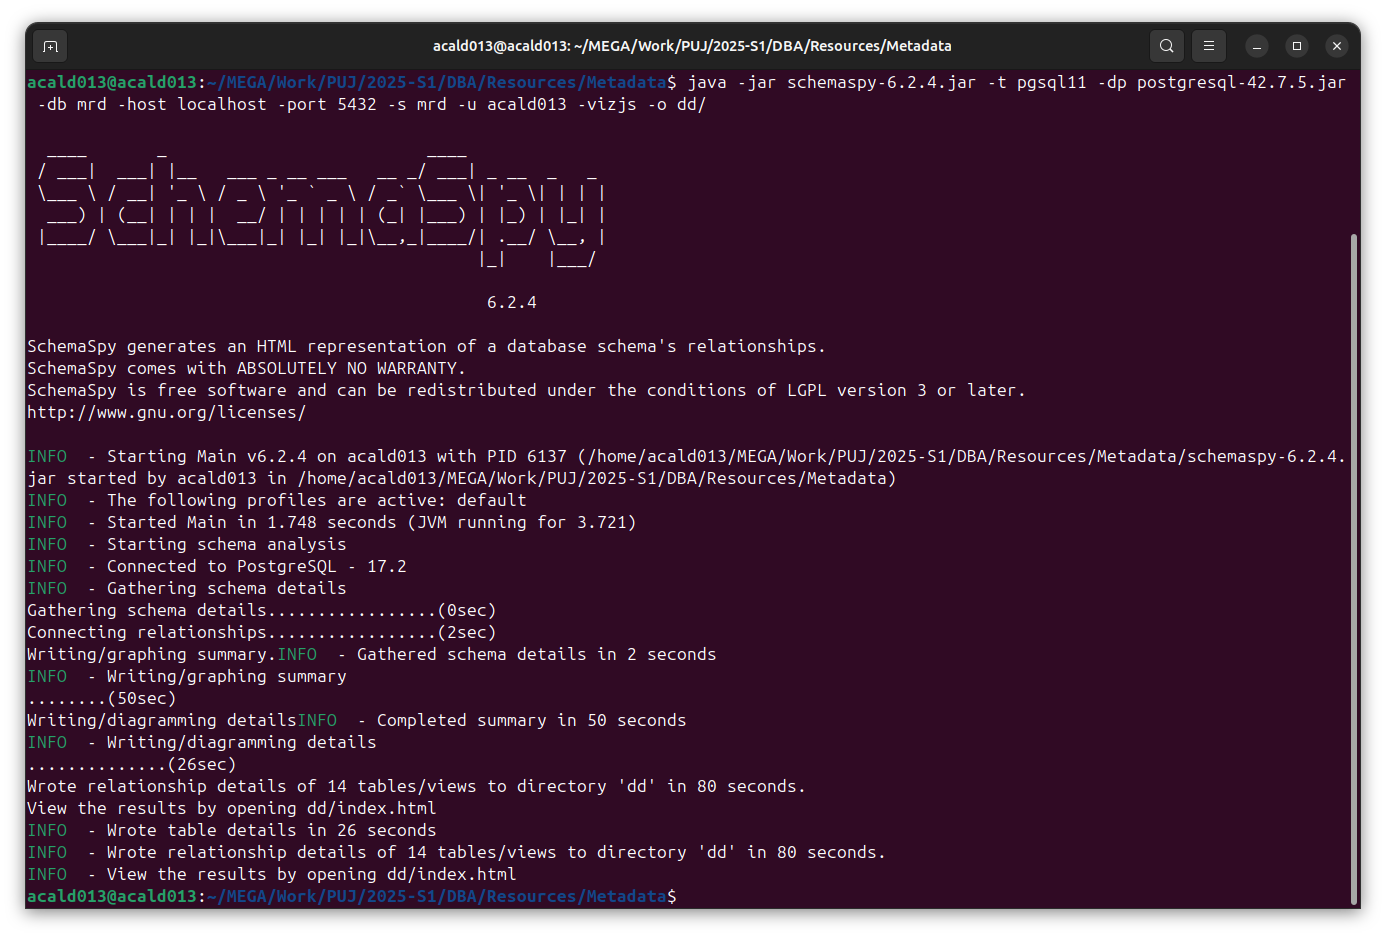
\includegraphics[width=\textwidth]{figures/output.png}
        \caption{Output of \texttt{schemaspy} over the MRD (in our case the PostgreSQL JDBC version should be 4.7.7).}
        \label{fig:output}
    \end{figure}

\end{enumerate}

\section{What is next?}

We expect two things from you and your team as independent work:

\begin{enumerate}
    \item As you can see in the \textit{Relationships} tab of the SchemaSpy Data Dictionary (DD) report for MRD, the relationships in the current database are implied. As stated in the report:

    ``\textit{No ``real'' Foreign Key relationships were detected in the schema. Displayed relationships are implied by a column's name/type/size matching another table's primary key.}''

    Your first task is to fix this issue by creating the appropriate integrity reference constraints for MRD. Specifically, all foreign keys must be defined according to the Entity-Relationship (E-R) Diagram shown in Figure \ref{fig:erd}.

    \item You will read the following \href{https://drive.google.com/file/d/1jqnAJ4A3AfnrTHHuYTcmOlaBXnUAznP1/view?usp=drive_link}{document} on metadata tools overview. It contains information about additional commercial and open-source tools that support metadata creation.

    Your task is to select one of these tools and create a similar tutorial, following the approach used with SchemaSpy, while analyzing the MRD data source. This should be done after updating the integrity reference constraints as required in the first task.
\end{enumerate}

We expect you to submit a well-structured report in PDF format, along with a dump file of the fixed MRD, packaged in a ZIP file, by \textbf{August 11, 2025}, via the link that will be provided on Brightspace.

\vspace{5mm}
Happy Hacking \includesvg[width=4mm]{figures/sunglasses}!

\end{document}

